\documentclass[oneside]{article}

% Package necessari
\usepackage[a4paper,top=2cm,bottom=2cm,left=1.5cm,right=1.5cm]{geometry}
\usepackage[utf8]{inputenc}
\usepackage[italian]{babel}
\usepackage[T1]{fontenc}
\usepackage{amsmath}
\usepackage{amssymb}
\usepackage{graphicx}
\usepackage[table, dvipsnames]{xcolor}
\usepackage{listings}
\usepackage{hyperref}
\usepackage{enumitem}
\usepackage{fancyhdr}
\usepackage{cancel}
\usepackage[ruled,vlined,linesnumbered]{algorithm2e}
\usepackage[noend]{algpseudocode}
\usepackage[font={small,sl}]{caption}
\usepackage[font={small,sl}]{subcaption}
\usepackage{tocbibind}
\usepackage{accents}
\usepackage[section]{placeins}
\usepackage{multicol}
\usepackage{mathtools}
\usepackage{dsfont}
\usepackage{color}
\usepackage{titlesec}

\usepackage{tcolorbox}

\makeatletter
\AtBeginDocument{%
  \expandafter\renewcommand\expandafter\subsection\expandafter{%
    \expandafter\@fb@secFB\subsection
  }%
}
\makeatother

% Colori per i listing
\definecolor{code_red}{rgb}{0.6,0,0} % strings
\definecolor{code_green}{rgb}{0.25,0.5,0.35} % comments
\definecolor{code_purple}{rgb}{0.5,0,0.35} % keywords
\definecolor{code_background}{rgb}{0.95,0.95,0.92} % background
\definecolor{verify_blue}{HTML}{12ACF2}
\definecolor{verify_red}{HTML}{F2122C}
\definecolor{verify_yellow}{HTML}{FFBB00}
\definecolor{dark_green}{rgb}{0.0, 0.5, 0.0}
\definecolor{dark_red}{rgb}{0.8, 0.0, 0.0}

% Stile del codice standard (C)
\lstset{
	language=C, 
	backgroundcolor=\color{code_background},
	frame=single,
	basicstyle=\ttfamily\small,
	keywordstyle=\color{code_purple}\bfseries\small,
	stringstyle=\color{code_red}\small,
	commentstyle=\color{code_green}\small,
	numbers=left,
	numberstyle=\small\color{gray},
	numbersep=5pt,
	tabsize=4,
	showtabs=false,
	showspaces=false,
	showstringspaces=false,
	escapechar=|, 
	captionpos=b,
	breaklines=true,
}

% Aggiunto paragraph come subsubsubsection
\setcounter{secnumdepth}{3}
\titleformat{\paragraph}
{\normalfont\normalsize\bfseries}{\theparagraph}{1em}{}
\titlespacing*{\paragraph}
{0pt}{3.25ex plus 1ex minus .2ex}{1.5ex plus .2ex}

% Impostazione delle lunghezze di alcuni elementi del documento
\setlength{\parskip}{1em}
\setlength{\parindent}{0em}
\setlength{\arrayrulewidth}{0.1em}

% Informazioni per la title page
\title{Network and System Defense}

\date{A.A. 2021/2022}

\author{Alessando Chillotti\thanks{\texttt{\href{mailto:alessandro.chillotti@outlook.it}{alessandro.chillotti@outlook.it}}}}

% Impostazione del package hyperref
\hypersetup{
    colorlinks=true,
    linktocpage=true,
    linkcolor=blue,
    urlcolor=blue,
    pdftitle={Network and System Defense},
    pdfauthor={A. Chillotti},
}
 
% Stile del codice standard (C)
\lstset{
	language=C, 
	backgroundcolor=\color{code_background},
	frame=single,
	basicstyle=\ttfamily\small,
	keywordstyle=\color{code_purple}\bfseries\small,
	stringstyle=\color{code_red}\small,
	commentstyle=\color{code_green}\small,
	numbers=left,
	numberstyle=\small\color{gray},
	numbersep=5pt,
	tabsize=4,
	showtabs=false,
	showspaces=false,
	showstringspaces=false,
	escapechar=|, 
	captionpos=b,
	breaklines=true,
}

\pagestyle{fancy}
\fancyhf{}
\lhead{\small A.Chillotti}
\rhead{\small Network and System Defense}
\cfoot{\thepage}
%\cfoot{Pagina \thepage}
\SetNlSty{bfseries}{\color{black}}{}

% Spaziatura tabelle
\renewcommand{\arraystretch}{1.5}

\graphicspath{ {./figs/} }
% Definizione del colore delle tabelle
\newcommand{\tablecolors}[1][2]{\rowcolors{#1}{yellow!50}{yellow!25}}

% Definizione dello stile da usare per la P di probabilità (grassetto in math-mode)
\newcommand{\pr}{\mathbf{P}}

% Forzatura del displaystyle in math-mode
\everymath\expandafter{\the\everymath\displaystyle}

%\newcommand{\scaption}[1]{\small{\caption{#1}}}
\renewcommand{\lstlistingname}{Snippet}

% Definizione di comandi per operatori matematici
\newcommand{\xor}{\oplus}

% Definizione osservazione
\newcommand{\obs}{\underline{Osservazione}}

% Definizione di \texttt{•} per matematica
\newcommand{\matht}[1]{\text{\texttt{#1}}}

% Definizione di domande e risposta
\newcommand{\question}[2]{
\textit{#1}\\
#2
}

\begin{document}
\maketitle
\tableofcontents
\newpage

\section{Traccia del progetto}
È richiesto produrre un payload (utilizzando qualunque vettore) che è in grado di installare una DNS shell (e.g. guardare \href{https://github.com/sensepost/DNS-Shell}{qui}) utilizzando un horsepill attack. Il payload deve essere in grado di sopravvivere agli update del kernel.

\section{Contesto dell'attacco}
L'attacco implementato all'interno del progetto si basa sull'idea di sfruttare l'\textit{init ramdisk} (\textit{initrd}). Esso è un memory-only file system che viene caricato in memoria dal kernel con lo scopo di svolgere alcune funzioni importanti:
\begin{multicols}{2}
\begin{enumerate}
\item Caricare i moduli necessari
\item Rispondere ad eventi di hotplug
\item Cryptsetup
\item Trovare e montare \textit{rootfs}
\item Fare il clean up di \textit{initrd}
\item Eseguire l'\textit{init} process
\end{enumerate}
\end{multicols}

L'attacco implementato cerca di costruire un \textit{init ramdisk} infetto che svolge le seguenti operazioni:
\begin{multicols}{2}
\begin{enumerate}
\item Caricare i moduli necessari
\item Cryptsetup
\item Trovare e montare \textit{rootfs}
\item Enumerare i thread kernel
\item Invocare \texttt{clone(CLONE\_NEWPID, CLONE\_NEWNS)}
\item Effetuare il remount di root
\item Montare uno scratch space
\item Effettuare una \texttt{fork()} nella quale si può fare l'hook degli aggiornamenti e si può implementare una backdoor shell
\item Invocare \texttt{waitpid()} per attendere l'\textit{init} process nel namespace
\item Effettuare lo shutdown/reboot del sistema
\end{enumerate}
\end{multicols}

Al passo 5 viene invocata una variante della \texttt{fork} che consente di specificare dei flag come \texttt{CLONE\_NEWPID} e \texttt{CLONE\_NEWNS} ed in questo caso si sta creando un namespace. All'interno del container vengono eseguite le seguenti operazioni:
\begin{multicols}{2}
\begin{enumerate}
\item Effettuare il remount di \texttt{/proc}
\item Costruire kernel thread fake
\item Fare il clean up di \textit{initrd}
\item Eseguire l'\textit{init} process fittizio
\end{enumerate}
\end{multicols}

\section{Implementazione dell'attaco}
\subsection{Costruzione dell'\textit{init ramdisk} infetto}
Per la costruzione dell'\textit{init ramdisk} infetto sono stati implementati i seguenti passaggi:
\begin{enumerate}
\item All'interno della directory \texttt{/tmp} viene estratto l'\textit{init ramdisk} presente all'interno del sistema originale con il seguente comando
\begin{tcolorbox}
\texttt{unmkinitramfs path-of-original-initrd path-to-initrd-extracted}
\end{tcolorbox}
\item Si effettua il download del codice sorgente della libreria \texttt{klibc}
\item Si applica la patch al sorgente scaricato al passo precedente attraverso l'utilizzo di \texttt{quilt}
\item Si utilizza il comando \texttt{dpkg-buildpackage} per costruire il pacchetto binario \textit{run-init}
\item Il binario \textit{run-init} generato al passo precedente viene inserito sotto il path \texttt{main/usr/bin/run-init} all'interno della directory in cui è stato inserito il risultato dell'estrazione performata al passo 1
\item Viene costruito l'\textit{init ramdisk} considerando l'estrazione eseguita al passo 1 modificata al passo 5 e, per eseguire questa costruzione, sono stati eseguiti i seguente comandi:
\begin{enumerate}
\item Aggiunta del primo microcode firmware
\begin{tcolorbox}
\texttt{cd early} \\
\texttt{find . -print0 | cpio --null --create --format=newc > /tmp/infected-initrd}
\end{tcolorbox}

\item Aggiunta del secondo microcode firmware
\begin{tcolorbox}
\texttt{cd ../early2} \\
\texttt{find kernel -print0 | cpio --null --create --format=newc >> /tmp/infected-initrd}
\end{tcolorbox}

\item Aggiunta del ram filesystem
\begin{tcolorbox}
\texttt{cd ../main} \\
\texttt{find . | cpio --create --format=newc | lz4 -l -c >> /tmp/infected-initrd}
\end{tcolorbox}

Si può notare che è stato utilizzato l'algoritmo di compressione \texttt{lz4} con il flag legacy abilitato. Si è scelto di utilizzare l'algoritmo \texttt{lz4} piuttosto che l'algoritmo \texttt{lzma} perché attraverso l'analisi, effettuata mediante lo strumento \texttt{binwalk}, dell'\textit{init ramdisk} originale si è notato l'utilizzo di \texttt{lz4}. Quindi, questo ha permesso di mantenere un'aderenza significativa con l'\textit{initrd} originale. Inoltre, l'algoritmo \texttt{lz4} è molto più rapido nella computazione rispetto a \texttt{lzma}.
\end{enumerate}
\item Si sostituisce l'\textit{init ramdisk} originale con l'\textit{init ramdisk} infetto
\item Si effettua il reboot
\end{enumerate}

L'intera sequenza di passaggi viene eseguita da uno script che permette di automatizzare la generazione di un \textit{init ramdisk} infetto. Il file eseguibile è il file \texttt{infect.sh}.

\subsection{Definizione della patch utilizzata per la costruzione dell'\textit{init ramdisk} infetto}
\subsubsection{Struttura della patch \texttt{horsepill-attack.patch}}
La patch utilizzata al passo 3 della sotto-sezione precedente è rappresentata dal file \texttt{horsepill-attack.patch} ed è composta dalle seguenti parti:
\begin{itemize}
\item Modifica del file \texttt{klibc-x.x.x/usr/kinit/run-init/runinitlib.c}
\item Modifica del file \texttt{klibc-x.x.x/usr/kinit/run-init/Kbuild}
\item Inserimento del nuovo file \texttt{klibc-x.x.x/usr/kinit/run-init/horsepill.c}
\item Inserimento del nuovo file \texttt{klibc-x.x.x/usr/kinit/run-init/horsepill.h}
\item Inserimento del nuovo file \texttt{klibc-x.x.x/usr/kinit/run-init/dnscat.h}
\item Inserimento del nuovo file \texttt{klibc-x.x.x/usr/kinit/run-init/reinfect.h}
\end{itemize}

\newpage
\subsubsection{Modifica del file \texttt{klibc-x.x.x/usr/kinit/run-init/runinitlib.c}}
Il file \texttt{runinitlib.c} è stato modificato in modo tale che, prima dell'invocazione dell'\textit{init} process si passi ad eseguire in una porzione di codice facente parte dell'attacco. Infatti, oltre all'aggiunta della seguente linea di codice 
\begin{center}
\texttt{\#include "horsepill.h"}
\end{center}
il file \texttt{runinitlib.c} è stato modificato nel seguente modo:

\begin{tcolorbox}
{\color{dark_green}{\texttt{perform\_hacks();}}}\\
\texttt{execv(init, initargs);}\\
\texttt{return init;}
\end{tcolorbox}

In questa maniera, prima di far partire l'esecuzione dell'\textit{init} process viene invocata la funzione \texttt{perform\_hacks()} facente parte del file \texttt{horsepill.c}.

\subsubsection{Modifica al file \texttt{klibc-x.x.x/usr/kinit/run-init/Kbuild}}
È stato modificato il file \texttt{Kbuild}, ovvero è il \texttt{Makefile} ed esso contiene delle regole di compilazione come i file oggetto da includere. Infatti, poiché è stato inserito il file \texttt{horsepill.c}, il file \texttt{Kbuild} ha subito i seguenti cambiamenti:
\begin{tcolorbox}
{\color{dark_red}{\texttt{-objs := run-init.o runinitlib.o}}}\\
{\color{dark_green}{\texttt{-objs := run-init.o runinitlib.o horsepill.o}}}
\end{tcolorbox}

\subsubsection{File \texttt{klibc-x.x.x/usr/kinit/run-init/dnscat.h}}
La DNS shell utilizzata è la \texttt{dnscat2} ed il file \texttt{dnscat.h} è un file header che contiene solamente due variabili:
\begin{itemize}
\item la variabile \texttt{dnscat} che è un vettore di \texttt{unsigned char} ed esso contiene il codice binario del file eseguibile del client di \texttt{dnscat2};
\item la variabile \texttt{dnscat\_len} che è un \texttt{unsigned int} e contiene la dimensione del vettore di \texttt{unsigned char}.
\end{itemize}

L'esistenza di questo file permette, a run-time, la scrittura del contenuto (byte per byte) del file client di \texttt{dnscat2}. Il file client originale è disponibile all'interno del repository GitHub di \texttt{dnscat2}\footnote{\url{https://github.com/iagox86/dnscat2}}.

\subsubsection{File \texttt{klibc-x.x.x/usr/kinit/run-init/reinfect.h}}
Il file \texttt{reinfect.h}, in modo similare al file \texttt{dnscat.h}, contiene un array di \texttt{unsigned char} che rappresenta il contenuto, byte per byte, di un file eseguibile ed una variabile che contiene il numero di byte dell'array. L'array rappresenta il contenuto byte per byte dello script \texttt{reinfect.sh}, ovvero uno script creato ad-hoc per permettere la reinfezione della macchina a valle di un aggiornamento.

Per la conversione da file eseguibile a contenuto byte per byte è stato scritto un comando ad-hoc:
\begin{tcolorbox}
\texttt{hexdump -e '16/1 "0x\%02x, " "\textbackslash n"' file}
\end{tcolorbox}

Lo script \texttt{reinfect.sh} è simile allo script \texttt{infect.sh}, ma utilizza il \textit{run-init} salvato all'interno dello scratch space e quindi non necessita di utilizzare la rete per scaricare la libreria \texttt{klibc}.

\subsubsection{File \texttt{klibc-x.x.x/usr/kinit/run-init/horsepill.c}}
Il file \texttt{horsepill.c} contiene gli elementi principali dell'attacco. L'entrypoint è rappresentato dalla funziona chiamata \texttt{perform\_hacks()} ed essa performa le seguenti operazioni:
\begin{enumerate}
\item Enumerazione dei thread kernel

In questo passaggio si sono acquisite informazioni tramite il file system \texttt{proc} poiché contiene una gerarchia di file speciali che rappresentano lo stato corrente del kernel. Per ogni file si va a leggere il contenuto di \texttt{/proc/\#proc/stat} e si ottengono informazioni come \texttt{pid} e \texttt{pid name}.
\item Invocazione della \texttt{clone(CLONE\_NEWPID, CLONE\_NEWNS)}

È stata create una funzione wrapper che incapsula la raw interface della \texttt{clone}, ovvero la 
\begin{center}
\texttt{\_\_clone(int flags, void* sp)} 
\end{center}
definita in \texttt{klibc/usr/include/sched.h}. L'invocazione della funzione wrapper ritorna il valore del \texttt{pid} ed in base al suo valore ci sono due possibili casi distinti.
\end{enumerate}

Nel caso in cui stia eseguendo il reale \textit{init} process vengono eseguite le seguenti operazioni:
\begin{enumerate}
\item Si monta lo scratch space nel path \texttt{/lost+found} con permessi \texttt{755}
\item Viene effettuato il remount del root

Questo viene effettuato perché solitamente il root è read-only a questo stage.
\item Si salva il \textit{run-init} infetto all'interno dello scratch space
\item Si scrive il contenuto byte per byte del file \texttt{reinfect.sh} nel path \texttt{/lost+found/reinfect}
\item Viene spawnato il processo che si occupa dell'implementazione di hook sugli update
\item Si scrive il contenuto byte per byte del client di \texttt{dnscat2} nel path \texttt{/lost+found/dnscat}
\item Viene spawnato il processo che si occupa dell'implementazione della backdoor shell passandogli come argomenti l'indirizzo IP del server, la porta e la secret
\end{enumerate}

Nel caso in cui stia eseguendo l'\textit{init} process vittima eseguirà i seguenti passaggi:
\begin{enumerate}
\item Viene effettuato il remount di \texttt{proc}
\item Vengono creati i thread kernel fake

Vengono eseguite una serie di \texttt{fork} ed attraverso una funzione ad-hoc, per ogni thread, vengono eseguite le seguenti operazioni:
\begin{enumerate}
\item Si apre, in modalità lettura, il file \texttt{/proc/self/stat} per fare il retrieve delle informazioni \texttt{arg\_start} (l'indirizzo sopra il quale gli argomenti di command line sono posizionati) e \texttt{arg\_end} (l'indirizzo sotto il quale gli argomenti di command line sono posizionati)
\item Se l'area di memoria non è sufficiente ne viene allocata una nuova
\item Vengono settate le informazioni di cui è stato fatto il retrieve tramite la funzione \texttt{prctrl} con l'utilizzo dei flag \texttt{PR\_SET\_MM\_ARG\_START} e \texttt{PR\_SET\_MM\_ARG\_END}
\item Se le operazioni al passo precedente sono andare a buon fine, viene settato il nome del thread sempre con l'invocazione della funzione \texttt{prctl}, ma con il flag \texttt{PR\_SET\_NAME}	
\end{enumerate}
\end{enumerate}

Inoltre, l'hook per gli update è stato realizzato grazie al costrutto \texttt{inotify}. Per implementare l'hook è stato definito un \texttt{watch} che, nel path \texttt{/boot/}, notifica gli eventi di tipo \texttt{IN\_MOVE}. La tipologia d'evento da notificare è stata scelta grazie alla creazione di un programma che ha l'obiettivo di notificare tutti gli eventi che avvengono nel path \texttt{/boot/} a seguito dell'esecuzione del seguente comando:
\begin{center}
\texttt{sudo update-initramfs -u -k all}
\end{center}
L'output prodotto dal programma è il seguente:
\begin{figure}[ht!]
\centering
\frame{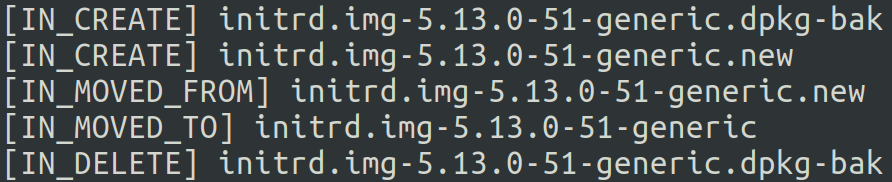
\includegraphics[width=0.6\textwidth]{figs/inotify}}˘
\caption{Eventi notificati dopo l'esecuzione di \texttt{update-initramfs}}
\end{figure}

\newpage
Quindi, il processo di reinfezione ha inizio nel momento in cui viene notificato l'evento \texttt{IN\_MOVE\_TO} dell'\textit{init ramdisk} aggiornato. In particolare, viene lanciato lo script \texttt{reinfect} in modo tale da infettare il nuovo \textit{initrd} andando ad utilizzare il \textit{run-init} salvato all'interno dello scratch space.

\subsection{Preparazione del server \texttt{dnscat2}}
Dalla repository GitHub di \texttt{dnscat2}\footnote{\url{https://github.com/iagox86/dnscat2}} sono stati scaricati i file necessari per l'esecuzione del server. Il server \texttt{dnscat2} viene messo in esecuzione, una volta che si risiede all'interno della directory \texttt{server}, con il seguente comando:
\begin{center}
\texttt{bundle exec ruby dnscat2.rb --dns `host=X.X.X.X,port=53531'}
\end{center}

\section{Simulazione dell'attacco}
L'attacco è stato eseguito sfruttando l'interconnesione fra due macchine virtuali collegate alla stessa rete locale.\\ Le macchine in questione presentano le seguenti caratteristiche: 
\begin{itemize}
\item l'utilizzo del sistema operativo \textit{Ubuntu 20.04.2} con la versione kernel \textit{5.13.0-40-generic};
\item una svolge il ruolo di client, ovvero rappresenta la macchina vittima dell'attacco;
\item una svolge il ruolo di server, ovvero rappresenta la macchina che attende connessioni sulla shell \texttt{dnscat2} da parte della macchina client.
\end{itemize}

\section{Struttura della directory di progetto}
Il repository GitHub\footnote{\url{https://github.com/alessandrochillotti/horsepill-attack}} ha la seguente struttura:
\begin{itemize}
\item \texttt{horsepill-attack.patch}: è il file che contiene la patch che, se applicata, consente la costruzione del \textit{run-init} infetto;
\item \texttt{src}: contiene i file sorgenti che costituiscono l'attacco
\begin{itemize}
\item \texttt{dnscat.h}
\item \texttt{horsepill.c}
\item \texttt{horsepill.h}
\item \texttt{reinfect.h}
\end{itemize}
\item \texttt{scripts}: directory contenente gli script creati
\begin{itemize}
\item \texttt{infect.sh}: la sua esecuzione implementa l'infezione della macchina vittima;
\item \texttt{reinfect.sh}: la sua esecuzione implementa l'infezione della macchina vittima a valle di un aggiornamento.
\end{itemize}
\item \texttt{README.md}: mostra un how-to per svolgere l'attacco.
\end{itemize}

\end{document}
